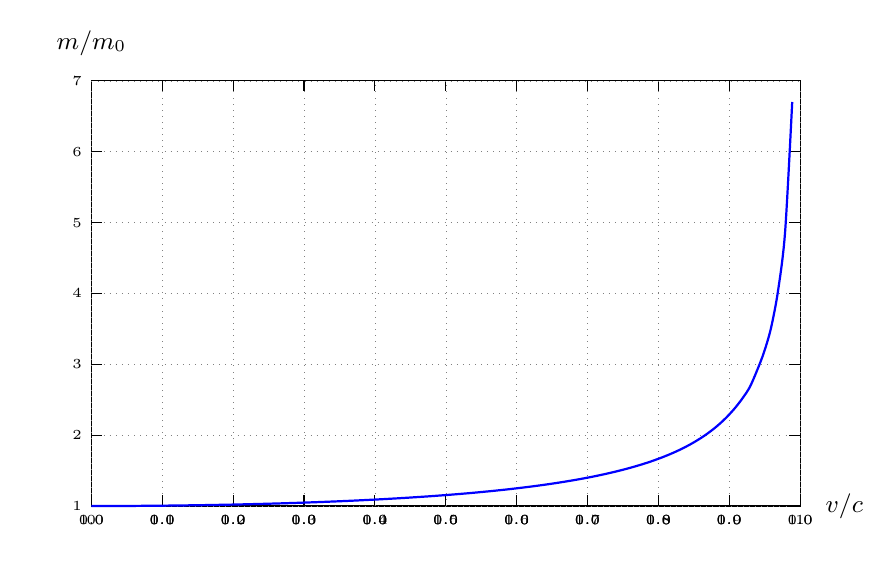
\begin{tikzpicture}[scale=0.9]
    
\tikzset{axi/.style={thin}}
\tikzset{aux/.style={very thin,gray,dotted}}

\clip (-0.9,-0.5) rectangle (10.9,6.75);

\draw[axi] (0,0) coordinate (A) rectangle (10,6) coordinate(B);

\foreach \x in {0,1,...,10}
{
    \draw[aux] (\x,0) coordinate (X1) --(\x,6) coordinate (X2);
    \draw[axi] (X1) -- ++(0,+0.15);
    \draw[axi] (X2) -- ++(0,-0.15);
    \ifthenelse{\x=0}
    {
        \path (X1) node[below] {\tiny $0.0$};
    }
    {
        \ifthenelse{\x=10}
        {
            \path (X1) node[below] {\tiny $1.0$}; 
        }
        {
            \path (X1) node[below] {\tiny $\fpeval{\x/10}$};
        }
    }
}

\foreach \y in {0,1,...,6}
{
    \draw[aux] (0,\y) coordinate (Y1) --(10,\y) coordinate (Y2);
    \draw[axi] (Y1) -- ++(+0.15,0);
    \draw[axi] (Y2) -- ++(-0.15,0);
    \path (Y1) node[left] {\tiny $\fpeval{\y+1}$};
}

\path (B-|A) node[above=0.2cm] {\small $m/m_0$};
\path (B|-A) node[right=0.2cm] {\small $v/c$};

\draw[thick,blue] plot[domain=0:9.89,smooth,samples=100] (\x,{1/(1-(\x/10)^2)^(1/2)-1});

\end{tikzpicture}
